\cleardoublepage
\chapter{Background} \label{chapter:ch2}
\markboth{Background}{Background}
%\addcontentsline{toc}{chapter}{Background}


%---------------------------------------------------------------------------
% FUNCTIONAL MAGNETIC RESONANCE IMAGING
%---------------------------------------------------------------------------


Magnetic resonance imaging (MRI) is a powerful tool to characterise brain function non-invasively, and has proven a successful way to investigate the neurological substrate of clinical outcomes in young populations. 
In order to understand its capabilities as well as its limitations, it is important to understand the biophysical underpinnings of the technology. 
Thus, in this chapter, I initially introduce this technique and provide an overview of the related state-of-the-art analytical methods in Section \ref{sub:fMRI}, followed by an introduction on the clinical aspects of preterm birth in Section \ref{sub:preterm}. 
I then summarise currently available knowledge provided by brain imaging in the preterm population in Section \ref{sub:fMRI_in_preterm}.

\section{Magnetic resonance imaging (MRI) as a tool to investigate brain function} \label{sec:MRI}
Magnetic resonance imaging \citep{Lauterbur1973} of bodily tissues is a relatively young technique \citep{Damadian1977} which depends on a basic set of physics principles concerning the interaction of protons, radio frequencies and magnetic fields. The following is a summary of how it produces images of living tissues, such as the ones used in the studies presented in the next chapters --- for a detailed review see \citeauthor{Grover2015}, \citeyear{Grover2015}. 
The main element that enables the use of MRI technology for this purpose is hydrogen, due to its high concentration in all tissues. 
Each atom of this substance can be seen as a sphere carrying a positive charge and is always spinning along random orientations, which causes it to "wobble" (Figure \ref{fig:ch2_spins}A/B). 
Since moving charges produce a magnetic field, we can think of these protons as tiny bar magnets. 

In the presence of a strong magnetic field, such at the static magnetic field generated by the MRI machine (B\textsubscript{0}), the protons’ axes align with the field lines created by the magnet, creating a net magnetization (M\textsubscript{0}; Figure \ref{fig:ch2_spins}B). 
M\textsubscript{0} can be considered as a vector containing two components: A longitudinal component M\textsubscript{L},  parallel to B\textsubscript{0}; and a transverse component M\textsubscript{T}, perpendicular to it. 
The hydrogen nuclei’s spinning motion combined with an external force causes them to precess about B\textsubscript{0} with an angular frequency according to the Larmor frequency \citep{Larmor1897}, but at random phases. 
The time it takes for a proton to sweep out a ’cone’ once is called its resonance frequency. Different protons precess with different frequencies, and this property has an important role in informing their physical location. 
This is because gradient coils (X, Y and Z) create a secondary magnetic field which distorts B\textsubscript{0} in a predictable pattern, causing the proton’s resonance frequency to vary according to position. 
This is what allows the MR signal to be spatially encoded, currently to a resolution of 1\textendash3 mm.




\begin{figure}[h!]
\centering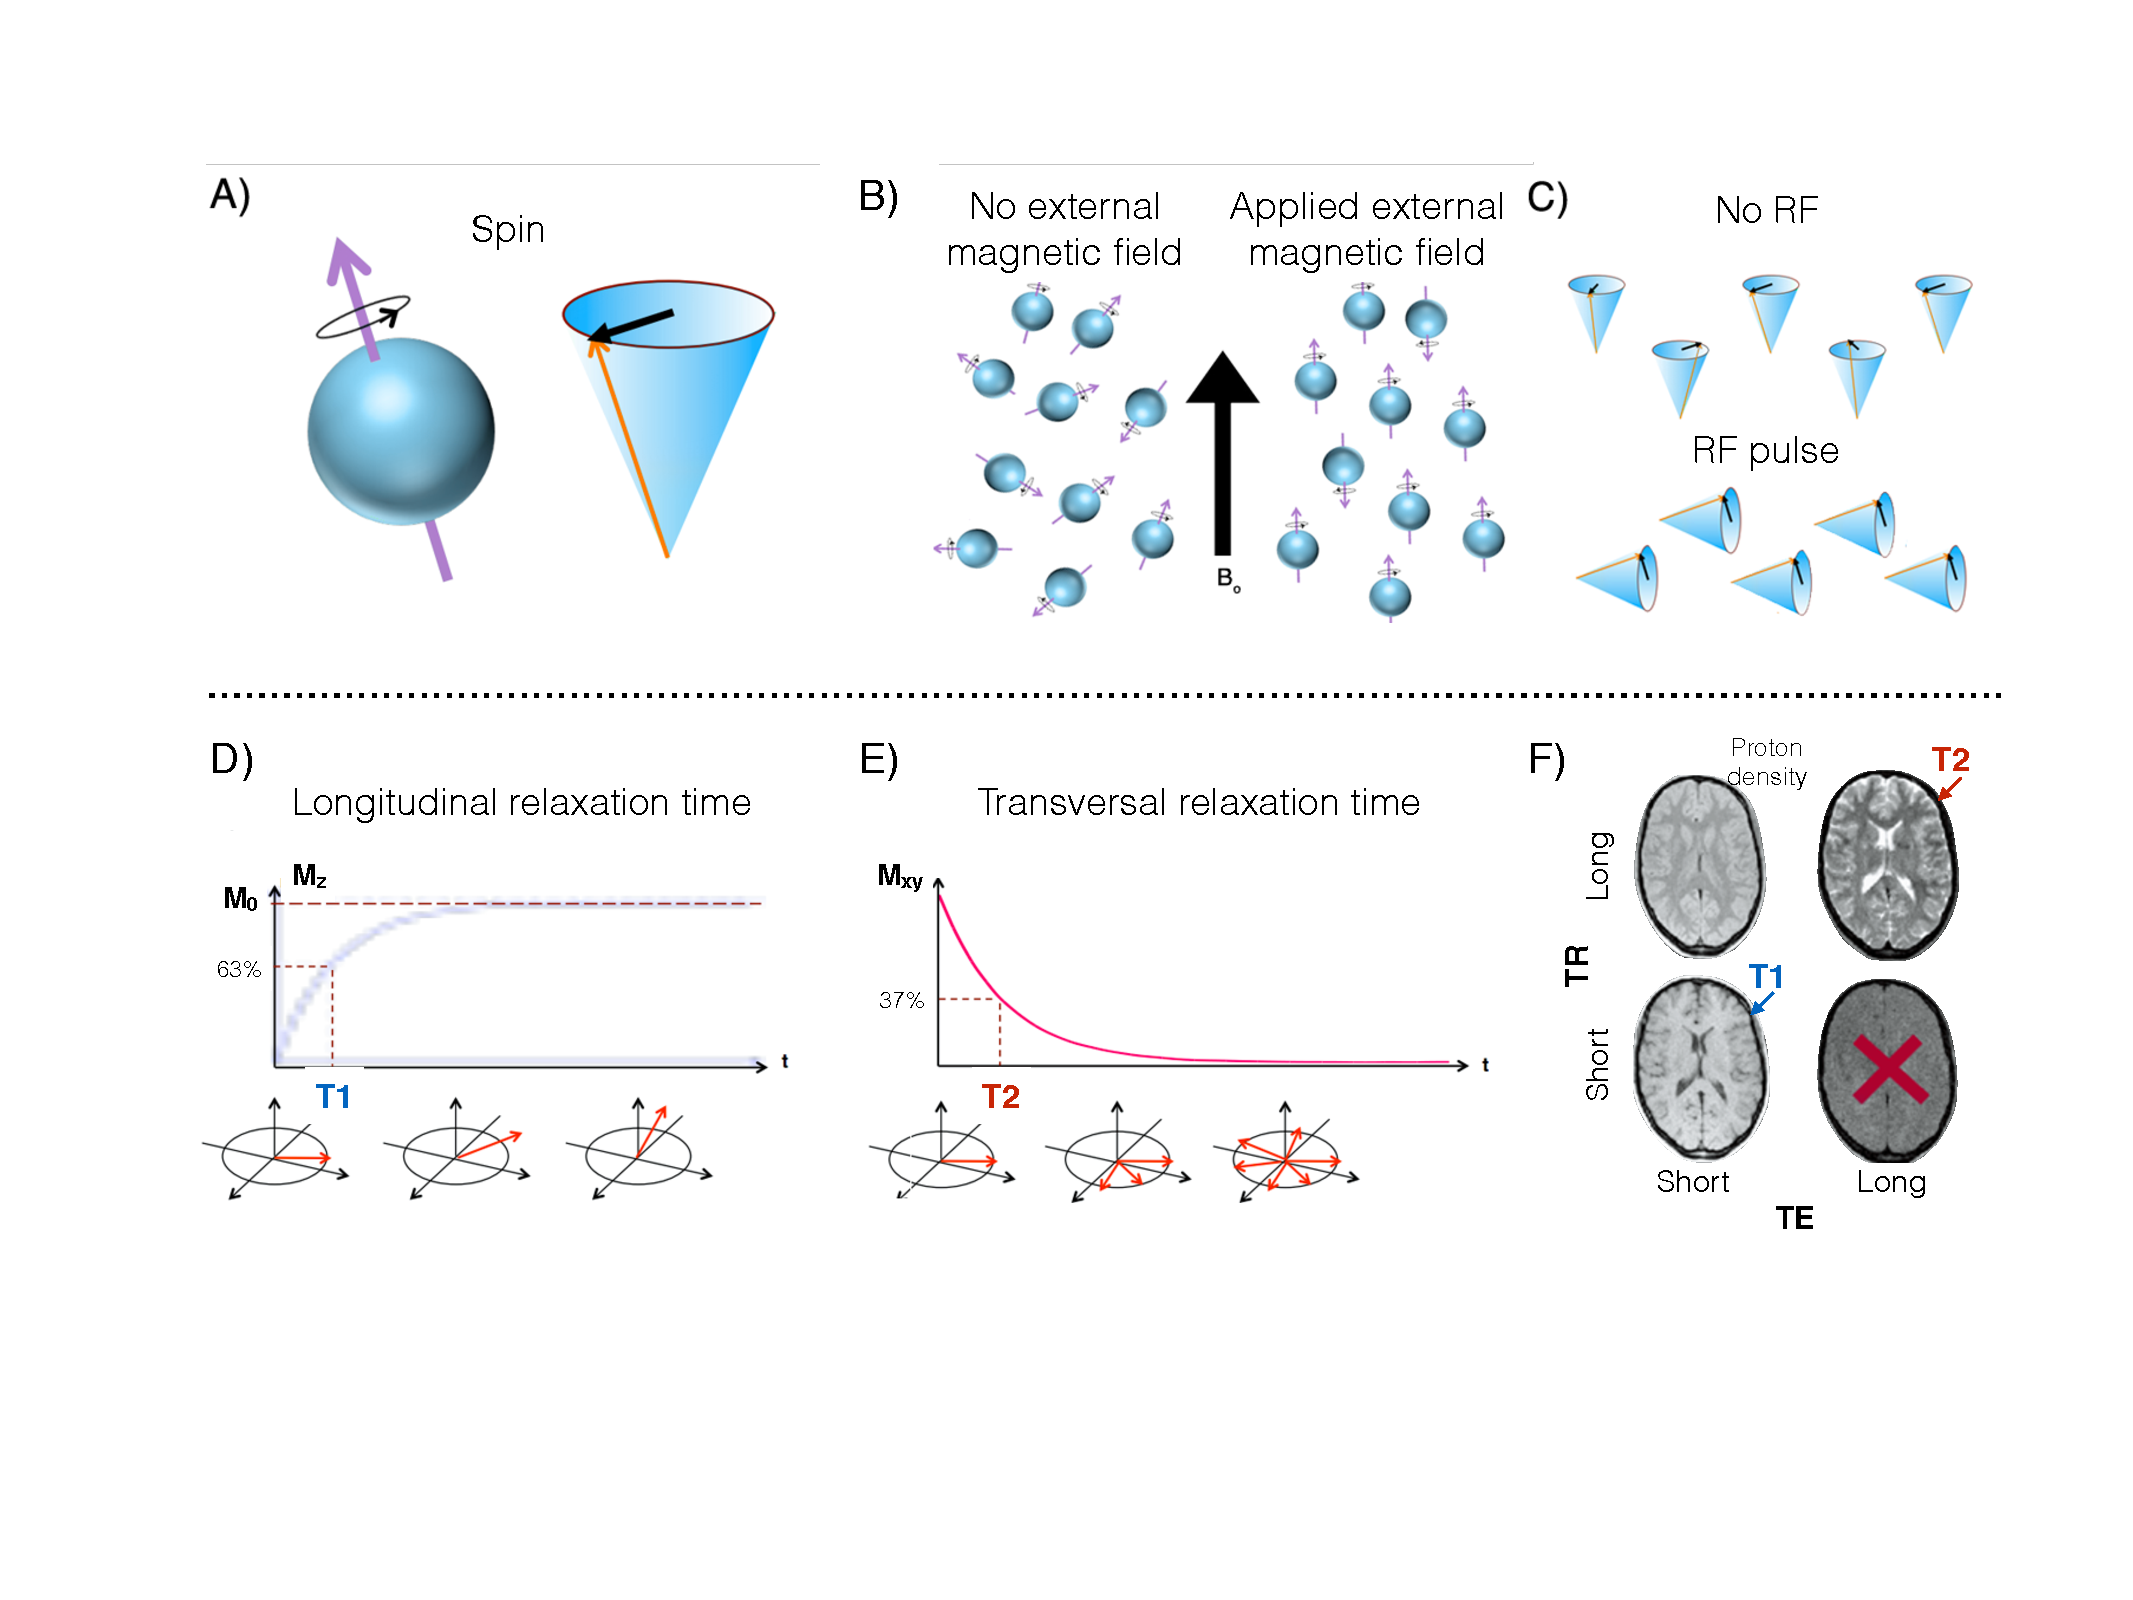
\includegraphics[width=1\linewidth]{images/Ch2/Ch2_spins.pdf}
\caption{\textbf{Magnetic resonance Imaging.} A)~A proton's spin. B)~ Alignment of protons in the present of a magnetic field B\textsubscript{0}, creating a net magnetisation M\textsubscript{0} which contains two components: a longitudinal M\textsubscript{L} which is parallel to B\textsubscript{0}; and a transverse component M\textsubscript{T} which is perpendicular to it. C)~When an electromagnectic radio frequency (RF) pulse transmitted by the RF coil present in the MR machine is applied, the hydrogen nuclei's phases align and they tip over, decreasing the longitudinal magnetisation and establishing a new transverse magnetisation. D)~when the RF pulse is stopped, the system slowly returns to equilibrium: the transversal magnetisation begins to disappear (transversal relaxation, described by time constant T\textsubscript{2}), while the longitudinal magnetisation returns to its original size (\textit{i.e.}, longitudinal relaxation, described by time constant T\textsubscript{1}). E)
~By altering the repetition (TR) and the echo time (TE), we can select the characteristic that we want to emphasise in the tissues.} \label{fig:ch2_spins}
\end{figure}




When an electromagnectic radio frequency (RF) pulse transmitted by the RF coil present in the MR machine is applied, the hydrogen nuclei's phases align and they tip over (Figure \ref{fig:ch2_spins}C), decreasing the longitudinal magnetisation and establishing a new transverse magnetisation. 
Then, when the RF pulse is stopped, the system slowly returns to equilibrium: the transversal magnetisation begins to disappear (a phenomenon called transversal relaxation, described by time constant T\textsubscript{2}), introduction of tissue in B0 will lead to small variations in magnetic field as a function of local magnetic susceptibility, while the longitudinal magnetisation returns to its original size (\textit{i.e.}, longitudinal relaxation, described by time constant T\textsubscript{1}) --- see Figure (\ref{fig:ch2_spins}D/E). 
This process creates a signal that can be measured by a receiver coil contained in the MR machine. 
A third property,  T\textsubscript{2}\textsuperscript{*}, describes the combined effect of local inhomogeneities (for example caused by field distortions near blood vessels which contain deoxyhemoglobin) and T\textsubscript{2} in the magnetic field. 
The MRI scanner can be programmed to emphasise the effects of those inhomogeneities, and this forms the foundation of blood oxygenation level dependent (BOLD) functional MRI, as discussed in the next section.

By altering how often an RF pulse is applied and the echo time (TE;  that is, the time between the onset of the RF excitation pulse and the highest signal induced in the coil), we can select the characteristic that we want to emphasise in the tissues (Figure \ref{fig:ch2_spins}F). 
The measured signal is then given by $M_0 (1-e ^{-TR/T_1} )e^{-TE/T_2^{(*)}}$,
where T\textsubscript{1} and T\textsubscript{2} are tissue properties, which allows representing boundaries between different brain tissues (namely gray and white matter, and cerebrospinal fluid, in the case of brain imaging).

 
 In addition to tissue localisation, information on spatial field inhomogeneities can be acquired using an MR machine, which may be an important asset when combining anatomical data with the functional images that we describe in the next section. This is because areas of boundaries between tissues are particularly susceptible to causing local field inhomogeneities which can hamper the signal acquisition. As described earlier in this section, the spatial localisation of the acquired signal is encoded by magnetic field gradients positioned in three dimensions. Local field inhomogeneities which interfere with the deliberate imaging gradients may thus cause the local field of view to be miscalculated, which leads to spatial distortion and causes changes in signal intensity. Luckily, if a field-map scan is acquired, it can be used in image post-processing steps to correct the occasional signal distortion. This can be done by acquiring two regular T\textsubscript{2}\textsuperscript{*}-weighted images acquired with different TE times, such that they produce different weightings. The phase-difference of the resulting signal from each voxel is linked to the 3 dimensional field variation in this voxel, which means post-processing algorithms are able to work out by how much each voxel needs to be "un-distorted" based on its field variation. While other methods exist for the acquisition of a field-map, this is the approach used for the all studies presented in this thesis. 

% TODO: FIELD MAP


%-----------------------
% FMRI BASICS
%-----------------------
\subsection{Functional magnetic resonance imaging (fMRI)}\label{sub:fMRI}


%- Describe fMRI data acquisition, what it can and cannot do. Show Elizabeth whatever's work with electrophysiology and fmri to show it reflects true brain activity. Focus on difficulties, especially for young populations. Talk about sinuses, movement, etc. 


The previous section provides an overview of the physical principles that enable the acquisition of a full image representing a brain volume, and is how the anatomical images used in this work are obtained --- the main goal now is to obtain images that reflect brain function across time.  To this end, the steps described in Section \ref{sec:MRI} are repeated every time a new image needs to be obtained, and the time between the acquisition of two volumes is called Repetition Time (TR). Typical fMRI studies use a TR of 2s but, especially more recently, this number has fallen to a bellow-second scale. 
By adjusting some of the parameters mentioned in the previous section, a sequence of images can be acquired that reflect brain function. 

After a number of preprocessing steps, which typically consist of motion correction; brain segmentation; co-registration; and spatial smoothing, fMRI images can be used to study intrinsic brain activity (resting-state fMRI) or brain responses to different stimuli (task-based fMRI). The results of brain activity investigations are usually shown in the form of maps that illustrate regions that activate or deactivate in a certain context. Since its beginning almost 30 years ago, fMRI has enabled a myriad of studies that greatly improved our understanding of the brain, as discussed in the next sections.


\paragraph{Interaction with physiology:} Functional brain imaging is possible thanks to the balance between energy needs from busy brain tissues and the blood flow that supplies those regions, which was discovered in the late 80's when \citeauthor{Ogawa1990} (\citeyear{Ogawa1990}) found that the blood's oxygenation level can be informative of cerebral activity.  

Active neurons require more oxygen and glucose to fuel its ion pumps than inactive cells. 
Those are supplied thanks to a link between neuronal activity and the heamodynamic response, called \textit{neurovascular coupling}. 
Most of the brain tissues are diamagnetic --- that is, they are repelled by the magnetic field. Haemoglobin, however, has two states: it is diamagnetic when oxygenated, but strongly paramagnetic (attracted by the magnetic field) when deoxygenated, as the release of oxygen from the molecule exposes the iron atoms' unpaired electrons. 
The latter creates inhomogeneities in (B\textsubscript{0}) and affects T\textsubscript{2}\textsuperscript{*} relaxation.
Thanks to this phenomenon, the measured blood oxygenation level dependent (BOLD) signals reflect the magnetic field’s inhomogeneities caused by these changes in oxygen levels in the blood.  
fMRI signals are, therefore, an \textit{indirect} measure of neuronal activity via its haemodynamic correlate. Several hypotheses have been proposed to explain the underlying mechanisms of neurovascular coupling \citep{Attwell2011}, but the exact nature of this complex link remains largely unknown \citep{Logothetis2004, Logothetis2008}.
However, the BOLD response has been shown to
be proportional to neuronal firing rates or population-level activity both using electrode implants \citep{Heeger2000}, optogenetics \citep{Lee2010, Kahn2011} and a combination of calcium imaging and two-photon microscopy \citep{Ma2016, OHerron2016}, among others. Figures \ref{fig:HRF} A and B illustrate the relationship between the haemodynamic response and neuronal activity after direct stimulation or under spontaneous conditions, respectively. % Hillman TODO


\begin{figure}[h!]
\centering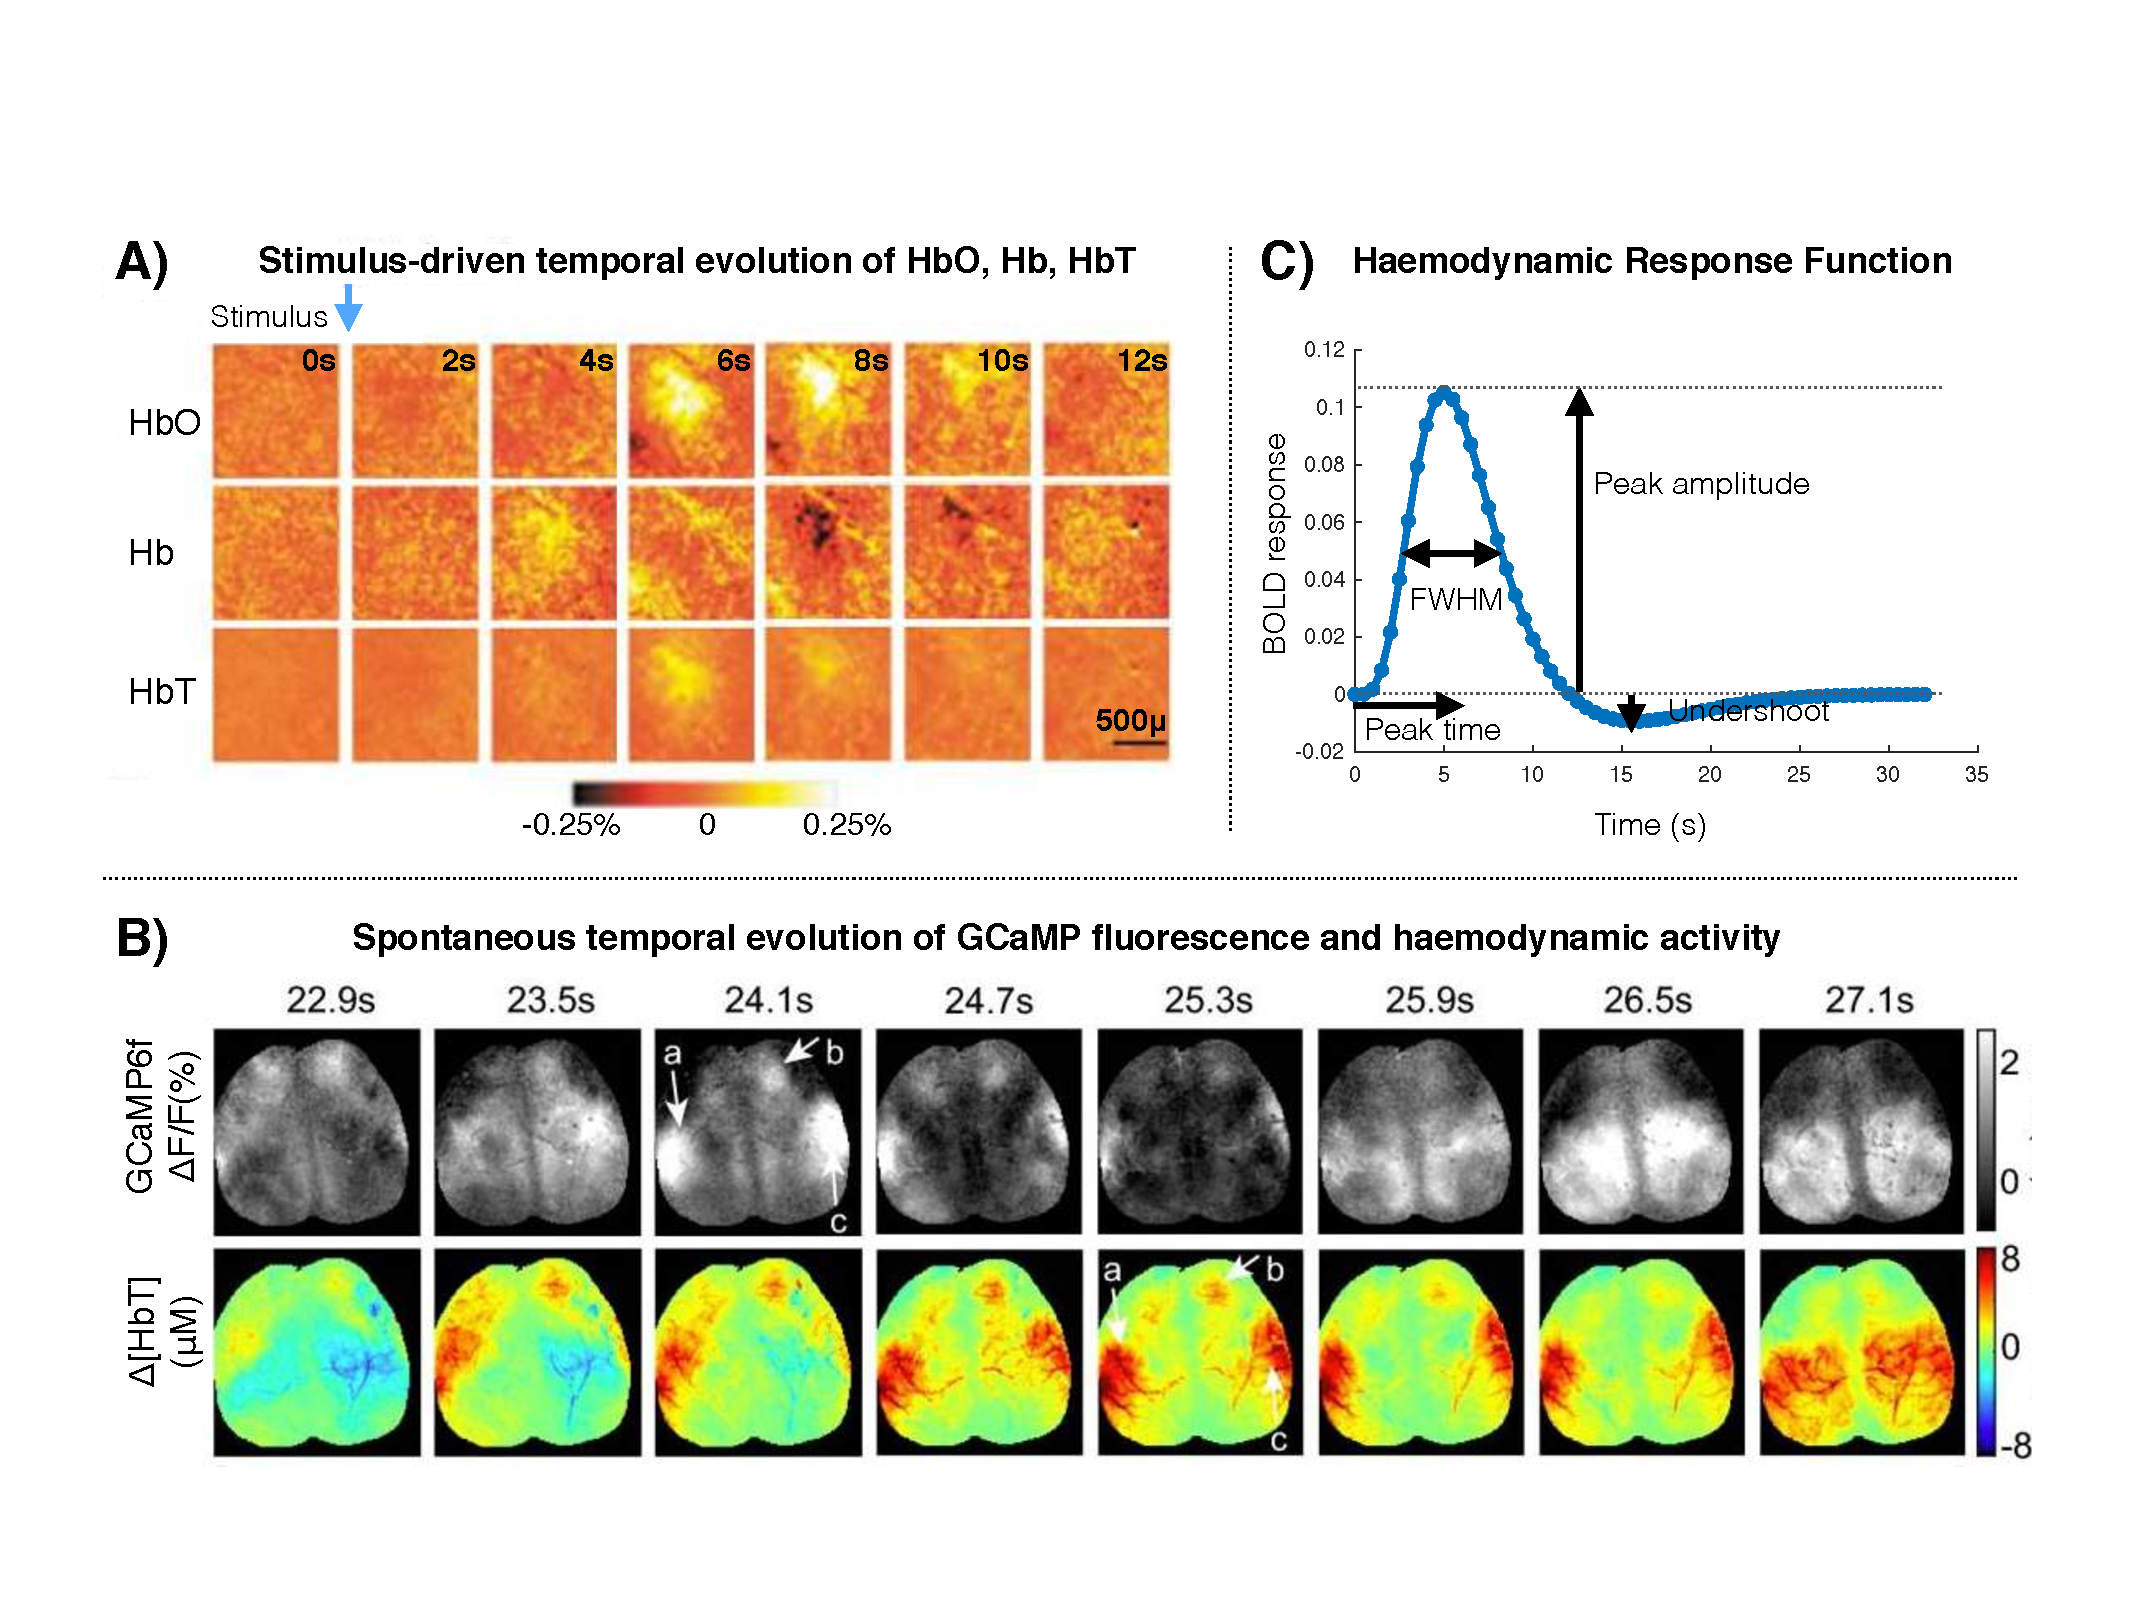
\includegraphics[width=1\linewidth]{images/Ch2/Ch2_HRF.pdf}
\caption{\textbf{The haemodynamic response and its link to neuronal activity.} A) Stimulus-driven spontaneous temporal evolution of oxygenated haemoglobin (HbO), deoxyhaemoglobin (Hb) and total haemoglobin (HbT, calculated as the sum of Hb and HbO) in the rat somatosensory cortex. Each image represents the average individual frame of 990 trials.  The Hb and HbO signals are expressed in percent change relative to baseline concentration (40 and 60 M, respectively). Image adapted with permission from \citet{Devor2003}. In this study, electrophysiological recordings of  local field potential (LFP) and multiple unit activity (MUA) were performed simultaneously to the haemoglobin measurements, revealing a strong non-linear relationship between the hemodynamic response and electrophysiological measures. B) Simultaneous imaging of \textit{(top)} wide-field imaging of GCaMP fluorescence (600 ms window average) and \textit{(bottom)} hemodynamic activity in the awake mouse brain without stimulation, showing comparable spatial patterns (a---c) with a time delay. Image taken with permission from \citet{Ma2016}. C) The so-called \textit{canonical} haemodynamic response function based on parameters reported by \citet{Friston1998}.  } \label{fig:HRF}
\end{figure}




It is important to note that the haemodynamic response (HRF) which enables BOLD signals to be measured is not instantaneous. Instead, it can be seen as a temporally blurred version of neural activity, due to the time course of neurovascular coupling, and peak response typically appears after a 5---6 s lag \citep{Menon2001,Logothetis2001}. The HRF is usually described by a combination of two gamma functions, peaking 6 s after stimulus delivery, followed by a negative overshoot peaking at 16 s, until it returns to baseline 20\textendash25 s post-stimulus, with a peak–undershoot amplitude-ratio of 6 (see Figure Figures \ref{fig:HRF}C). These numbers were obtained from a principal component analysis (PCA) of the data from \citet{Friston1998}, and are still widely used today. In general, it can be seen as a delayed and smoothed version of the underpinning neuronal activity. This is key for the steps that follow data acquisition, as accurately modeling the evoked haemodynamic response to neural events plays a crucial role fMRI data analysis \citep{Lindquist2009}.





% What it can do:
 % https://royalsocietypublishing.org/doi/full/10.1098/rstb.2015.0361


% What it can't do (Logothetis 2012):
    %That is, the fMRI signal cannot easily differentiate between function-speci c processing and neuromodulation or between bottom-up and top-down signals, and it may potentially confuse excitation and inhibition



% Elizabeth Hillman's papers:    https://www.ncbi.nlm.nih.gov/pmc/articles/PMC4147398/figure/F2/
   % RESTING STATE coupling between fMRI and neural activity: %https://www.pnas.org/content/113/52/E8463
   
   % TASK BASED coupling:
    % https://www.ncbi.nlm.nih.gov/pmc/articles/PMC5511559/
 



%-----------------------
% TASK FMRI
%-----------------------

\subsection{Task-based fMRI in the study of brain function}

A popular experimental design in functional studies is task-based fMRI (tb-fMRI). In this paradigm, participants are asked to repeatedly perform a specific task for a certain time (often referred to as a "block"), followed by a contrasting block (\textit{e.g.}, a "resting" period). By probing into BOLD signal differences between these conditions, it becomes then possible to identify parts of the brain which selectively activate or de-activate according to the task \citep{Friston1995a}.

\subsubsection{Static analysis of task-Based fMRI}

Task-based paradigms (as opposed to resting-state ones, see Section \ref{subsec:ch2_restingState}) rely on prior knowledge about external stimuli that may be driving brain activity. The most traditionally used approach to tb-fMRI analysis is the General Linear Model (GLM). This method examines the temporal synchrony between predicted responses and a voxel’s time series by modeling the latter as a linear combination of several factors that contribute to the signal \citep{Friston1995a}. In that way, the GLM is more flexible than, for example, a simple correlation analysis, in that it allows the inclusion as model factors of several experimental conditions, as well as of other known (\textit{e.g.}, motion parameters) or possible (\textit{e.g.}, behavioural information, subjects’ age, etc.) sources of variability. Typically, a comparison between task response is then done by subtracting conditions (\textit{e.g.}, task A - task B), or a factorial analysis is performed when the experimental design includes more than one factor (\textit{e.g.}, cognitive process). The statistical significance of the GLM’s results then reflects how well an experimental observation is fit by the model \citep{Worsley1995}. One of the drawbacks of this approach is that, although it reveals the magnitude of an effect, it does not provide information about its duration, nor is it possible to capture inter-subject differences in timing \citep{Robinson2009}. Nonetheless, this has been one of the most widely used methods in fMRI analysis with several applications and extensions being proposed \citep{Dale1999, Glover1999, Goldman2000, Laufs2003}.

From all GLM extensions, Psychophysiological Interaction (PPI) analysis is of particular interest here, as it concerns \textit{modulation} of functional connectivity. Originally proposed by \citeauthor{Friston1997} in \citeyear{Friston1997}, PPI determines which voxels enhance their relationship with a user-defined seed in a particular context (\textit{i.e.}, during a specific behavioural task). This is achieved by including at least three regressors in the model: 1)~the time course of the seed; 2)~the task time course; and 3)~the interaction regressor, calculated as an element-by-element multiplication of the seed’s activity and the task time courses. Including the first two guarantees that the variance explained by the PPI is over and above that explained by the task or by physiological correlations’ main effects \citep{OReilly2012a}. In that sense, voxels whose activity is well described by the interaction regressor (also called the PPI regressor) are those that have a stronger relationship with the seed during the task of interest. 

An alternative to these confirmatory analyses is to employ exploratory methods, which do not rely on prior knowledge. Principal component analysis, for example, can be used for dimensionality reduction by mapping the data into a reduced space that maximises the variance, and is often used as a first step in the fMRI analysis pipeline \citep{Zhong2009}. Of note, partial least squares (PLS) analysis \citep{Randal2004} maximises the co-variance between two modalities, making it possible to find links between multi-modal data (\textit{i.e.}, fMRI and behavioural data). By analysing task-related brain metrics in conjunction with behavioural or clinical outcomes, for example, this method makes it possible to characterise the neurological substrate of cognitive functions \citep{Roberts2017}.




%-----------------------
% RESTING STATE FMRI
%-----------------------

\subsection{Resting-state fMRI in the study of brain function} \label{subsec:ch2_restingState}

In the mid 90's, \citep{Biswal1995} showed in an original study that even at rest, activity in the motor cortex is remarkably structured and bilaterally coherent, despite the absence of an explicit motor task. Since then, resting-state functional magnetic resonance imaging (rs-fMRI) has become a widely used tool to investigate temporal fluctuations in neuronal activity by looking into  BOLD signals across the brain \citep{Damoiseaux2006, Fox2007}. Thanks to the absence of goal-directed stimulation or activity, this paradigm is particularly well suited for studying and comparing brain function between populations who might respond to task instructions with different levels of cognitive ability or attention such as clinical; ageing; or very young cohorts, because it has minimal compliance requirements. Additionally, provided that the same image acquisition parameters are used, this allows data recorded across multiple research centers to be pooled or compared, given that there is no variability task demands. These results are comparable even when the conditions slightly differ across studies (\textit{e.g.}, eyes closed; open; with or without fixation; etc.), so those can be appropriately chosen according to the comfort of the targeted population \citep{Soares2016}. Furthermore, this data can be acquired in a relatively short time, with sessions of 5\textendash7 min yielding a reasonable trade-off between acquisition time and the robustness of results in adults \citep{VanDijk2010, Whitlow2011}. In young children, 5.5 min has been shown to be an acceptable duration, to avoid head motion due to their becoming too restless \citep{White2014a}. 

In the preterm population, rs-fMRI has often been used in the context of functional connectivity (FC) analyses (see Section \ref{sub:static_rsfmri}), measuring temporal correlations between the activity of different brain regions or networks \citep{Lordier2019}. Thanks to these studies, it is now known that alterations in FC may begin even before birth \citep{Thomason2017} and often last through adolescence \citep{Wehrle2018} into adult life \citep{Papini2016}. 

\subsubsection{Static analysis of Resting-State fMRI} \label{sub:static_rsfmri}

Resting-state paradigms rely on intrinsic changes in brain activity for which no prior information is available, and so the most widely adopted approach to analyse these data has been to investigate temporal relationships between the spontaneous activity in different brain regions. Typically, this is achieved by looking into correlations between these time series over the entire duration of the scanning session. This method generally known in the literature as static functional connectivity (sFC), as it assumes those relationships are stable across time. It has been used to uncover correlations between all pairs of regions of interest (ROIs), unveiling the so-called functional connectome, or in seed-based analyses, to find correlation maps which illustrate all regions whose activity correlates with a chosen ROI \citep{Lee2013, Smitha2017}. 

These initial approaches led to the discovery that some of these relationships are recurrent and robust, such that several resting-state networks (RSNs) can be observed across subjects and experiments. A popular way to look into the static connectivity between these networks is independent component analysis \citep{McKeown1998, Calhoun2001}, a data-driven approach based on blind-source separation. It assumes that the signal from whole-brain voxels can be decomposed into groups of spatially and/or temporally independent signals, and these components can then be used to study within– or between–network correlations.   Figure \ref{fig:RSN} illustrates some of the networks that have been widely reproduced in different studies.





\begin{figure}[h!]
\centering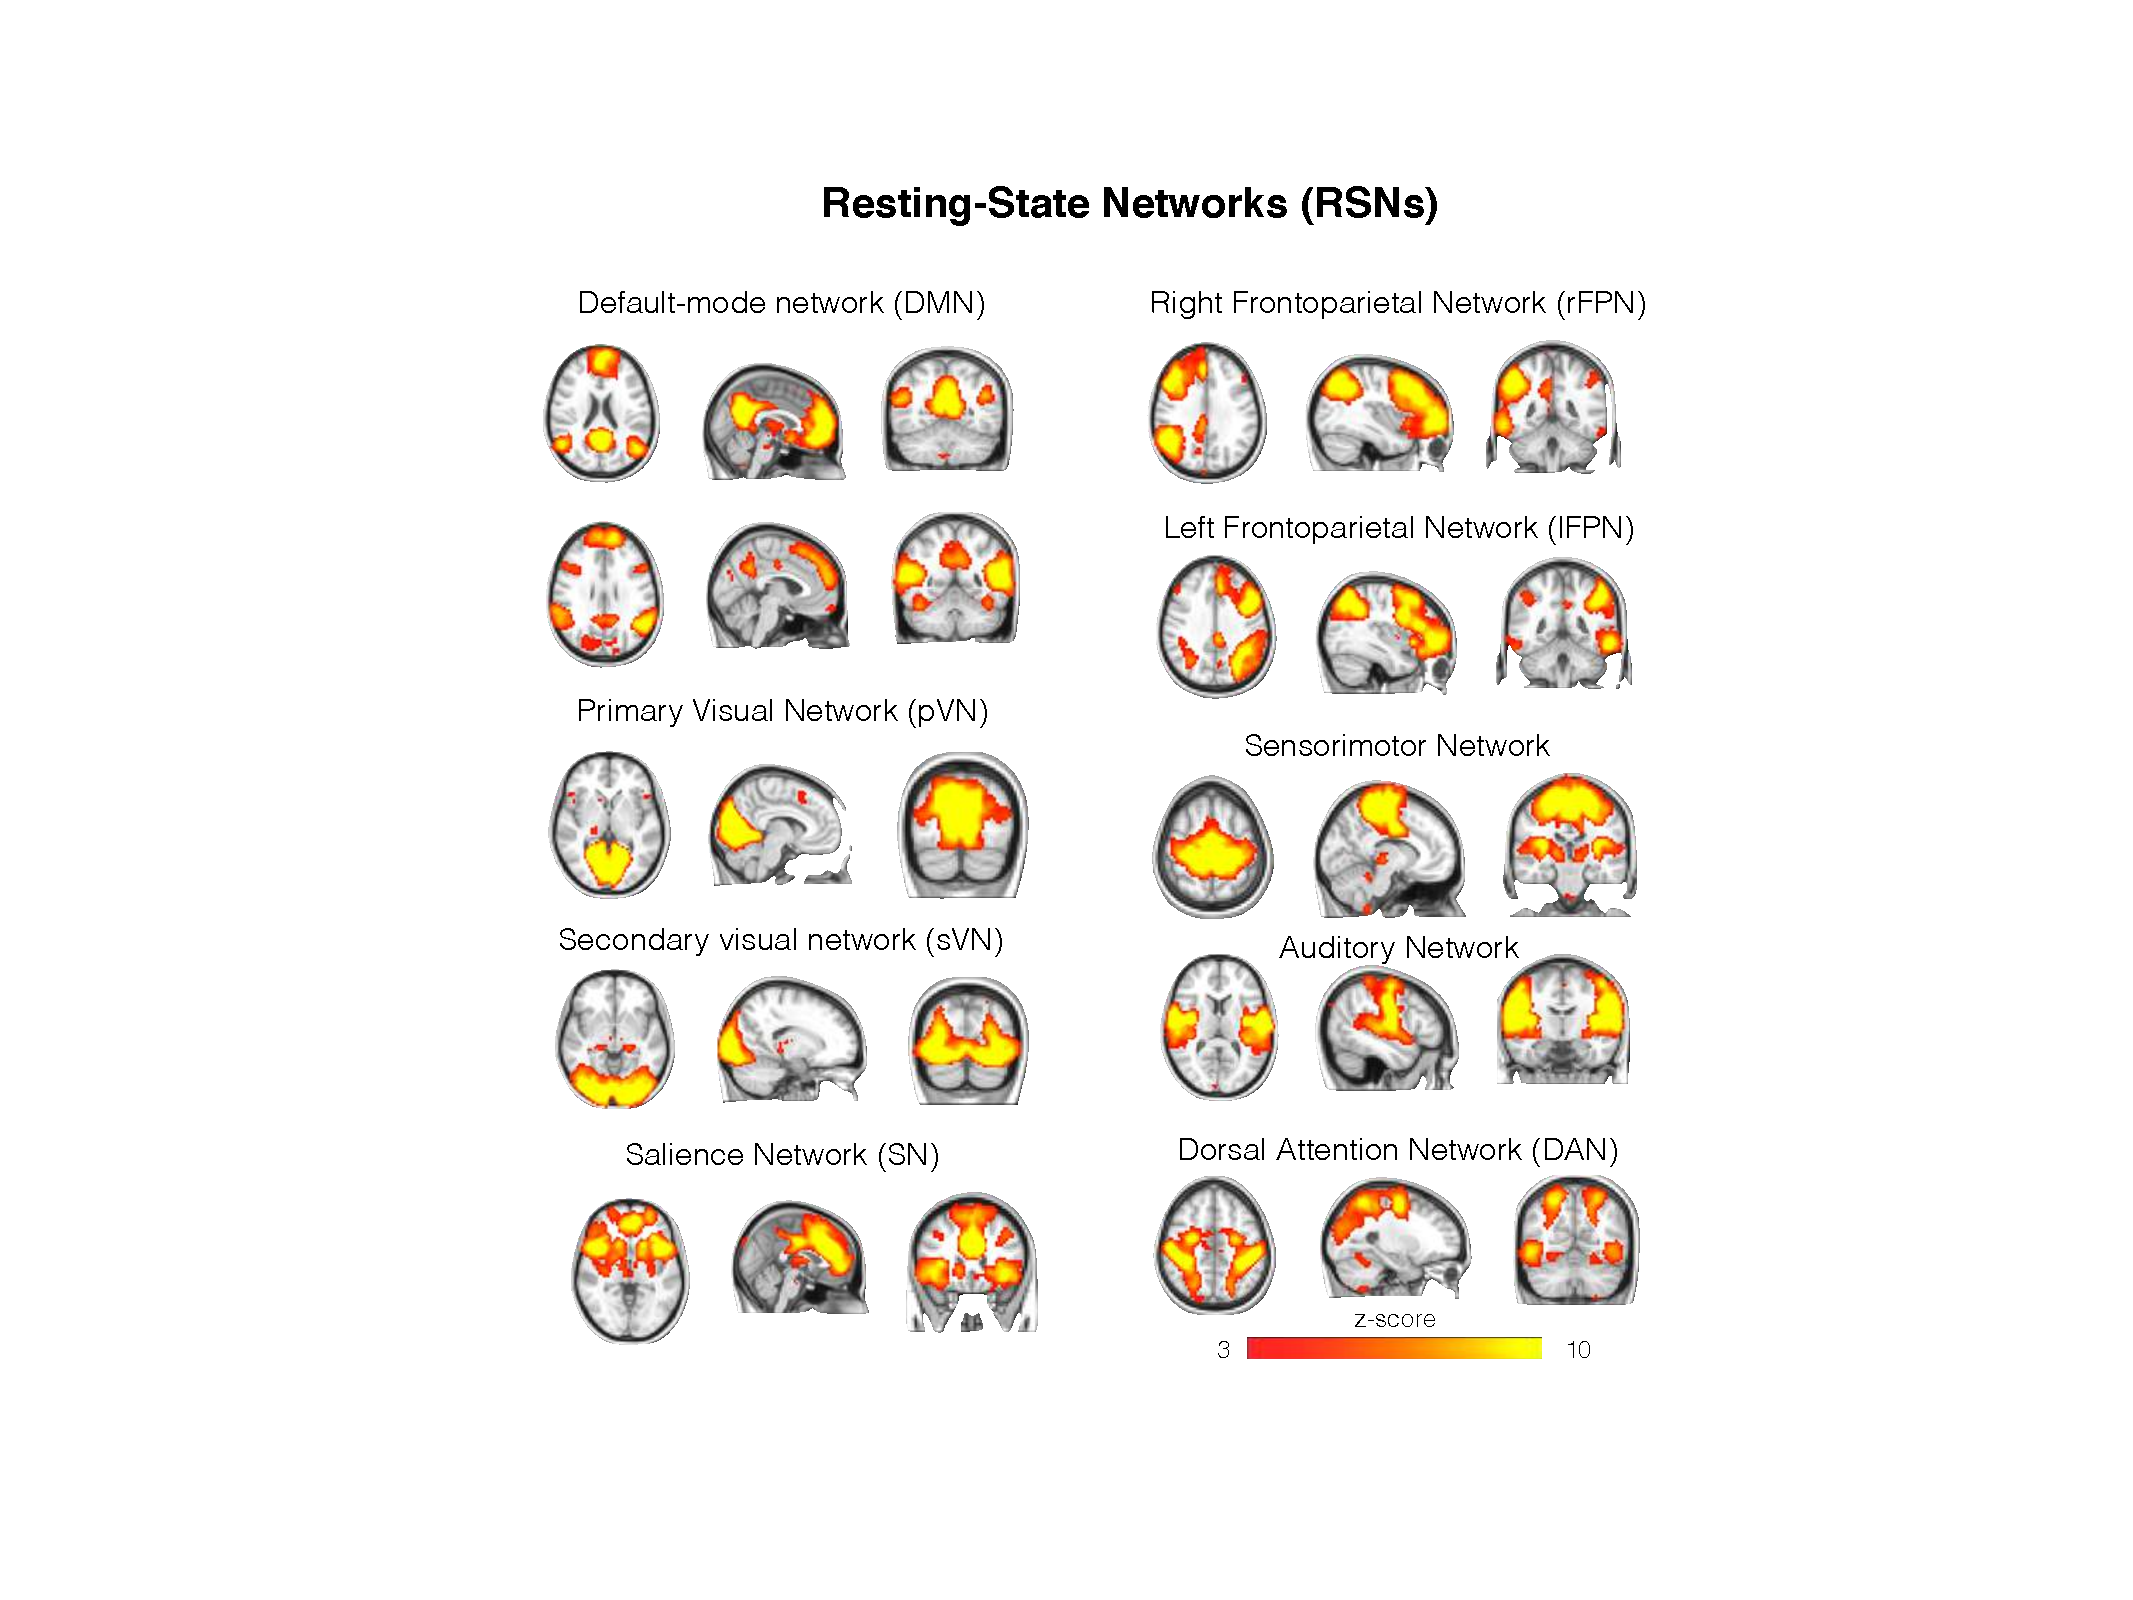
\includegraphics[width=0.9\linewidth]{images/Ch2/Ch2_RSN.pdf}
\caption{\textbf{The resting-state networks.} Some networks have been repeatedly reproduced in resting-state experiments. The ones illustrated above were obtained from an independent component analysis using data from 35 subjects. Figure adapted from \citet{Akbar2016}  } \label{fig:RSN}
\end{figure}





In an alternative method for brain network analysis, rs-fMRI can be seen in terms of graphs, where brain regions represent nodes and high correlation values represent edges \citep{Rubinov2010, Farahani2019}. The application of graph theory concepts in FC analysis reveals complex aspects of connectivity using graph parameters (\textit{e.g.}, nodal degrees, average path length, clustering coefficient, etc.) which complement traditional analysis methods. These metrics may then be used to shed light on the brain's ability to rapidly combine information from distributed regions, its resilience to external perturbations, among others.

\subsection{A dynamic approach to fMRI analysis}

\subsubsection{Dynamic analysis of Resting-State fMRI}


Although static methods are still the most widely-adopted approach for resting-state fMRI analysis, over the past decade a growing body of research has shown that FC is actually dynamic over time \citep{Chang2010}. Importantly, these time-varying properties of brain activity contain invaluable information to understand brain function \citep{Hutchison2013, Christoff2016}.

An initial parameter of brain dynamics is BOLD signal variability, usually calculated as the standard deviation of the BOLD time series at each voxel \citep{McIntosh2010}. Often overlooked as noise in traditional analyses, over the past decade it has been increasingly thought of as a potentially vital feature of brain function \citep{Garrett2010}, with higher variability seeming relevant to guarantee systems' stability and dynamic range \citep{Deco2011} as well as development and cognition in healthy \citep{Garrett2013} and clinical \citep{Zoller2017, Nomi2018, Easson2019} populations.

Besides the dynamics of brain activity, changes in the \textit{relationships} between different brain regions over time have also been increasingly found to be relevant, spawning the field now known as dynamic functional connectivity \citep{Hutchison2013, Preti2017}. The most popular approach quickly became using a sliding window, where the FC is typically computed over subsequent, temporally shifted windows to capture connectivity fluctuations \citep{Chang2010, Sakoglu2010, Kucyi2014}. This yields a series of FC matrices which contain the time courses of the fluctuation of pairwise correlations, and further analysis can then follow to detect dynamic brain states using a variety of additional methods such as principal component analysis \citep{Leonardi2013}, hidden Markov models \citep{Vidaurre2017}, etc. Despite its prominence, this framework remains limited by its dependence on window parameters, its inherently lowered temporal resolution \cite{Leonardi2015}, and its sensitivity to outliers since all time points within a window are given equal importance \cite{Lindquist2014}.

An alternative approach to sliding windows focuses on performing a point process analysis (PPA) by looking into subsets of single fMRI frames instead of focusing on entire time courses. This is possible because, when averaged, frames where a selected seed region is highly active reveal a pattern containing all regions that co-activate with that ROI \citep{Tagliazucchi2012}. This can be seen as a computationally efficient proxy of a seed-based static FC described in section \ref{sub:static_rsfmri}. As described above, however, FC patterns are known to be variable over time, and so a natural development of the PPA approach is to temporally cluster these selected frames into co-activation patterns (CAPs; \citeauthor{Liu2018}, \citeyear{Liu2018}). Each CAP is then a dynamic building block of the overall connectivity map, each varying in duration, number of appearances, etc. Going a step further, innovation-driven CAPs (iCAPs) cluster frames based not on similarity between patterns of \textit{activation}, but between patterns of activation  \textit{changes} \citep{Karahanoglu2015a}. The interest here lies in finding groups of regions whose activation change (activate or deactivate) simultaneously, allowing for temporal and spatial overlaps.     

\subsubsection{Dynamic analysis of task-Based fMRI}

Similar to the resting state, activation time courses upon the execution of a task are also known to show exquisite complexity that cannot be captured by standard stationary approaches \citep{Gonzalez-Castillo2018}. Although dynamic FC has increasingly become a natural avenue for resting-state research \citep{Preti2017}, task-based experiments have not yet fully benefited from this approach: only a few studies so far have explicitly investigated task-related dFC using fMRI \cite{Braun2015, Di2015, Simony2016}. \cite{Di2015}, for example, used sliding windows to calculate the Time-Varying Correlation Coefficient (TVCC) between different regions’ activities and found substantial fluctuations in FC patterns during stimulation periods. The method allowed them to observe a decrease in FC between visual areas shortly after stimulation onset, followed by a return to baseline. The disadvantages of this approach are twofold: firstly, the TVCC estimation is, as expected, dependent on the choice of window size; and secondly, to account for the low signal-to-noise ratio of the BOLD signal, the technique involves averaging each subject’s experimental blocks, which may be at the expense of relevant variability in FC dynamics. However, this study provides additional evidence that explicitly tracking connectivity pattern transients is paramount to advance our understanding of how different brain areas dynamically communicate in a task context. As expected from their importance in resting state, time-varying properties of brain activity during task performance have been recently shown to also contain relevant information to understand cognition \citep{Fong2019}. Taken together, the above corroborate the idea that moment-to-moment FC dynamics contain relevant information about behaviour, and thus promise to hold considerable translational value \citep{ Gonzalez-Castillo2018}.

%---------------------------------------------------------------------------
% PREMATURITY 
%---------------------------------------------------------------------------

\section{Preterm birth}\label{sub:preterm}

A birth is defined as preterm (PT) when delivery occurs after less than 37 completed gestational weeks, in contrast to the expected duration of 40 weeks, on average, in a healthy pregnancy. This can be further characterised as a moderate to late PT (32---36 weeks), very PT (28---31 weeks),  or extremely PT ($\leq$ 27 weeks). These conditions have been associated with a wide range of behavioural, cognitive and neuropsychological difficulties that have been identified at various stages in life. In the sections below, I provide an overview of the challenges brought by preterm birth to the child, their family, and society as a whole. I then explain the problems preterm-born individuals are at higher risk of facing later in life, the body of knowledge that has been build to date around the neural mechanisms for their clinical problems, and identify a gap in the literature regarding investigations of dynamic brain function in this population, which this thesis aims to fill. 


\subsection{The global challenge of prematurity}

Every year, an estimated 15 million babies are born too soon around the world, representing 5–18\% of all births depending on the country. 
Especially in the more extreme cases, complications related to an early birth are the leading cause of death among children up to 5 years old, and these complications are responsible for the loss of approximately 1 million infants each year \citep{Liu2016}. 
Although PT birth may be caused by various reasons and several well known biological pathways leading to it exist \citep{Behrman2007}, the majority of the cases are "idiopathic", meaning that it happens spontaneously and without an obvious cause.
Importantly, the number of PT births has been on the rise over the past 20 years \citep{Costeloe2012}, possibly as a consequence of  an increase in maternal age and changes in obstetric practices. 
Additionally, with the continuous improvements in medical treatment, the rates of survival have also increased across the world, meaning that more and more children will live with the effects of prematurity each year. 
Besides the consequences to the children's health and behaviour, this increase is expected to escalate the economic impact of PT birth not only in the short term (\textit{i.e.,} immediate medical care), but also in the longer term. 
In fact, according to the Institute of Medicine of the National Academy of Sciences, special education services related with a higher prevalence of disabling conditions in PT-born children cost U\$1.1 billion yearly in the United States alone, while the lost household and labour market productivity had an impact of approximately U\$5.7 billion \citep{Behrman2007}. % https://www.ncbi.nlm.nih.gov/books/NBK11358/





\subsection{Behavioural consequences of preterm birth}

Preterm birth puts children at a considerably higher risk of developing a broad range of cognitive deficits \citep{Brydges2018, Twilhaar2018}. % \Vandewouw et al, Human Brain Mapping, 2019
By school age, up to 50\% of these children develop cognitive, language, or socio-emotional disabilities that are likely linked to neurological abnormalities starting before birth, lasting through life and into adulthood \citep{Gozzo2009, Chaminade2013, Moiseev2014, Hornman2016, Thomason2017, Burnett2018}.

A meta-analysis of cognitive outcomes in more than 7000 children and teenagers born very preterm and aged 5--20 years old found that this population showed significant deficits in intelligence \cite{Twilhaar2018}. A similar study by \citet{Brydges2018}, involving more than 6000 individuals, showed that they scored significantly lower on intelligence tests; measures of executive functioning; and processing speed, as compared to their term born peers across a wide range of ages (4--17). This study found no association between the children's age at assessment and cognitive impairment, indicating that very preterm born children fail to catch up with term born ones throughout childhood and adolescence. In that sense, it seems that the differences between the two groups are due to a deficit in PT children, rather than a delay \citep{Brydges2018}. This is in line with \citep{Linsell2018}'s study, which found that cognitive function did not recover or deteriorate between infancy and adulthood in extremely preterm individuals, and explain why \cite{Doyle2010} find long-lasting effects of extremely preterm birth in an adult cohort. Importantly, socio-economic status at birth has been shown to affect IQ scores in adults born very preterm \citep{Breeman2017}, and to modify the relationship between early-life events and neurodevelopmental outcomes in preterm born children. Further understanding these complex relationships may shed light into potential avenues for promoting improved outcomes for infants at higher risk of neurodevelopmental issues \citep{Benavente-Fernandez2020}. 

Besides difficulties in executive functions, children who were born prematurely are also at a higher risk for socio-emotional disabilities \citep{Zmyj2017}, with impaired interactions being present in relationships with family, teachers and friends \citep{Twilhaar2019}. In particular, PTB children are less likely to initiate and respond to peers' efforts to participate in joint attention \citep{Zmyj2017}, which may aggravate later social cognition impairments and thus hinder social interaction skills. Whether these differences in social competences are a product of faulty or delayed maturation remains a topic for debate: some studies point towards the former hypothesis, since these effects have also been found in individuals through adolescence  \citep{Healy2013, Saigal2016}; while others put it down to a maturational lag, with findings that PTB children catch up with their full term peers by the age of 5 \citep{Witt2018}. These inconsistencies emphasise the complexity of the effects of preterm birth and the importance of further characterising the link between brain and behaviour.

The most recent research indicates cognitive control impairment as a central basis for social problems in PTB adolescents \citep{Twilhaar2019}. This finding further highlights the importance of understanding the neural substrate of cognitive disabilities in this population, with a view to detecting potential targets for early intervention. 

%- Emotion - attention - theory of mind - social adjustment (twilhaar J pediatr. 2019)
% Theory of mind: https://www.ncbi.nlm.nih.gov/pubmed/30342224
% Social Adjustment: https://www.ncbi.nlm.nih.gov/pubmed/31402139
% Social cognition: https://www.ncbi.nlm.nih.gov/pubmed/28611695
%Emotion Regulation: https://www.ncbi.nlm.nih.gov/pubmed/31056820

\subsection{Consequences of preterm birth on brain structure}

To identify potential interventions that would be able to recover some of the behavioural difficulties mentioned above it is important to, first, understand how the brain is affected by preterm birth. The brain undergoes significant growth and development in the last months of gestation, which naturally puts preterm-born infants at a considerably greater risk for abnormal neurodevelopment. A great body of research has thus been dedicated to understanding the consequences of prematurity on brain structure.

The most common pathology affecting babies born very preterm is the encephalopathy of prematurity, which is characterised by a subtle brain injury followed by disrupted brain growth and the development of internal (such as basal ganglia and thalamus) and external (cerebral cortex) structures \citep{Kunz2014}. In addition, prematurity has been associated with reduced white matter volume and myelination, decreased cortical grey matter as well as lower hippocampal, basal ganglia and cerebellar volume that lasts through childhood and adolescence. Moreover, these alterations have been linked to poorer neurodevelopmental \citep{Inder2005,Ment2009,Nosarti2013,Padilla2015} and educational \citep{Cheong2013} performance across childhood.

 Recently, studies have investigated regional volume changes and how they relate to specific neuropsychological consequences of preterm birth. Reduced dorsal prefrontal cortex (dPFC) volume was found to be linked to children's attention and hyperactivity problems \citep{Bora2014}. In adolescents, volume changes in the fusiform and orbitofrontal cortices have been associated with socialisation problems \citep{Healy2013}, and autism \citep{Johnson2014}. A reduction in hippocampal volume has also been shown to correlate with memory deficits in preterm children. Taken together, these studies emphasise the vulnerability of the brain after preterm birth.

Most neuroimaging studies involving preterm young adolescents rely on structural features, relating brain volumes or microstructure to clinical and cognitive outcomes \citep{Huning2018, Groeschel2019, Boardman2020}. While these structural studies provide relevant insights into brain injuries that are associated with prematurity and potentially underlie neurocognitive dysfunction, they cannot provide information on brain activation driven by specific demands. Studies that investigate brain function are thus necessary to provide complementary information on the consequences of preterm birth, as discussed in the next section.




\subsection{Consequences of preterm birth on brain function}

% Neural correlates of theory of mind: https://onlinelibrary.wiley.com/doi/full/10.1002/hbm.23750

% Neural of social stuff: 10.1016/j.jpeds.2013.08.011

% Neural characteristics of socio-emotional processin.

With the wide range of behavioural alterations related to PT birth, it is no surprise that the brain may be deemed more vulnerable to dysfunction in children who are born too early. 
A recent meta-analysis involving more than sixty-four thousand children found that prematurity of any degree affects neurodevelopment, and that these adverse effects persist at various follow up stages \citep{Allotey2018}. 



Several studies have investigated structural differences in preterm-born children \citep{Huppi1998b, Brown2014, Kersbergen2014, KostovicSrzentic2019}, but functional activation and connectivity has only been popularised in this population over the last decade, with studies primarily relying on resting-state static analysis. 
Fransson et al. (\citeyear{Fransson2007}) were the first to show the presence of resting-state networks (RSNs) in the preterm, which were later found to be similar to those found in adults \citep{Doria2010}. 
Notably, different RSNs formed at different rates during gestation. Many studies identified an incomplete set of RSNs in preterm subjects at term-equivalent age, although not all compared them to term-born controls \citep{Lin2008, Fransson2007, Fransson2011, Gao2015, Lordier2019}.
Additionally, alterations in the functional connectivity between and within RSNs were found in infants \citep{Gozdas2018} and adolescents \citep{Wehrle2018} born very preterm , providing evidence for the long-lasting impact that very PT birth has on the organisation of the brain \citep{Damaraju2010,White2014,Johns2019}. 

Common to all of the studies mentioned above, was the stationary aspect of the analysis and the use of a resting-state approach. 
Given the high incidence of cognitive abnormalities in preterm born children at a later stage, the study of brain function under specific cognitive tasks in this cohort is highly desirable, albeit largely lacking at present.

\subsection{Interventions for preterm newborns and children}

Early interventions are usually implemented shortly after birth, often relying on improving the care-giving environment and with the goal of subsequently improving clinical outcomes. They typically involve the family, including following integrative programs such as the Newborn Individualized Developmental Care and Assessment Program (NIDCAP; \citeauthor{Peters2009}, \citeyear{Peters2009}); the Infant Behavioral Assessment and Intervention Program (IBAIP; \citeauthor{VanHus2016}, \citeyear{VanHus2016}); the Victorian Infant Brain Studies (VIBeS PLus; \citeauthor{Spittle2018}, \citeyear{Spittle2018}); or using Kangaroo Mother Care position and method \citep{Peters2009}. A meta-analysis of these family-centred interventions has shown that they have a positive effect on cognition in children born very preterm, accompanied by a positive but weaker impact on motor abilities, and inconclusive results on language \citep{Ferreira2020}. Importantly, although these interventions have been beneficial, the exact environmental factors responsible for enhancing brain development remain largely unknown. 

Socio-emotional and executive function skills are still in plain development during childhood and adolescence, suggesting that this age may still be within the intervention window. There has been growing evidence that children's capacity to understand emotions affects their social adjustment. Those who are more sensitive to emotional cues tend to have better relationships with friends and adults, are less likely to present behavioural problems, are more inclined to solve conflicts, and tend to perform better at school \citep{Denham2006,Domitrovich2007, Harrington2020}. Socio-emotional training has been shown to reduce aggressive behaviour and to improve both emotion recognition and executive functions in typically developing children and children from disadvantaged families, providing further evidence for the link between different cognitive abilities \citep{Pons2002,Sprung2015, Grazzani2018, DeMooij2020}. In recent years, mindfulness meditation training has emerged as a potential tool to help young populations manage a wide variety of symptoms including disruptive behaviour \citep{Perry-Parrish2016}. A study involving typically developing children at 11 years old showed that 8 weeks of mindfulness training already has the potential to improve attentional self-regulation \citep{Felver2017}. Another, found that meditation programs can enhance cognitive and social-emotional development in young populations \citep{Schonert-Reichl2015}. Taken together, these results further suggest a link between these cognitive domains and that mindfulness meditation may be an avenue for intervention in clinical populations. In fact, several studies have investigated the benefits of a meditation-based intervention for children with attention deficit hyperactivity disorder, but their varying methodological quality means that so far no clinical recommendation can be made and further, well-designed analyses, must be performed \citep{Evans2018}.

Crucially, a recent neuroimaging study involving typically developing, fullterm-born, early adolescents found that mindfulness meditation related to dynamic features of brain function and network connectivity over time, as opposed to static characteristics of neural activation\citep{Marusak2018}. This brain function trait remains largely unexplored in preterm-born early adolescents, which highlights the importance of this thesis to fill this gap.


% Joana's music paper https://www.ncbi.nlm.nih.gov/pubmed/31765804

%---------------------------------------------------------------------------
% FUNCTIONAL DYNAMICS IN PREMATURITY (?) 
%---------------------------------------------------------------------------

\section{FMRI in the study of prematurity}
\label{sub:fMRI_in_preterm}


Thanks to recent advances in the field, fMRI has been increasingly used to characterise healthy brain function at different stages in life \citep{Power2010}. 
One important extension of these investigations is to understand alterations related to atypical neurodevelopment. 
This may lead to interventions aimed at preventing, reverting or minimising the effects of altered brain function.


FMRI is particularly well-suited to investigate paediatric populations, especially since robust measures of functional activation and connectivity can be obtained from short scanning sessions. It has been employed to uncover atypical connectivity patterns and their links to a wide range of neurodevelopmental disabilities. For instance, this technique has exposed altered brain responses in regions underlying executive functions in preterm-born children in frontal \citep{Reveillon2013,Murner-Lavanchy2014} and temporal areas \citep{Kwon2014a, Wilke2014} which were linked to impaired language performance at age 14\textendash15 \citep{Wilke2014}.

Most of the studies to date, however, employ analytical methods that assume brain function to be static --- that is, they investigate averaged brain activity across the entire experiment. Given that the brain is known to be highly dynamic, there is an urgent need to know how prematurity affects the dynamic features of neural function. The aim of this thesis is thus to fill this gap.



\subsection{Challenges and considerations for paediatric MRI studies}


MRI studies often require that participants lay completely still for lengthy periods of time, especially when the experimental protocol includes several imaging modalities or task paradigms. Head movement is one of the most intractable and potentially harming confounds in this type of data, causing misalignment of subsequent frames and, as a consequence, BOLD signal or structural estimates that do not correspond to true effects \citep{Friston1996,Siegel2017}. Compared to adults, children have decreased inhibitory control \citep{Bedard2002}, and may thus find it harder to remain still during experiments, particularly  given the distracting environment of scanning sessions \citep{Greene2016}. Unsurprisingly, then, children and adolescents tend to present much higher total head motion than adult participants \citep{Satterthwaite2013b}, making the data potentially more susceptible to results that do not reflect reality \citep{Power2012}. Motion scrubbing has become and increasingly accepted --- and stringent --- way of dealing with this type of artefact over recent years \citep{Power2014a,Laumann2016}, but when the data is highly affected by motion it leads to significant data loss. The best approach is, therefore, to avoid movement as much as possible.

Unsurprinsingly, head motion in fMRI experiments involving children tends to increase with the duration of experiments both in terms of run and session time \citep{Engelhardt2017}. While taking breaks between sessions has been suggested as a way to reduce run length-related artefacts, a trade-off must be found between implementing these and keeping the total recording time as short as possible \citep{Meissner2019}.  Another design-related consideration that influences head motion in child studies is the experimental paradigm \citep{Yuan2009a}. Children are less likely to move when they have something to pay attention to, such as in task-based experiments, as compared to resting-state ones \citep{Engelhardt2017}. Given the above, a potentially reasonable trade-off for protocols that include both types of experimental paradigms would be to perform the resting-state session as early as possible, and task-based sessions in sequence, all while trying to keep the total scanning time as short as possible. 


An approach that has been increasingly agreed as a measure to reduce head motion or drop-outs due to scanner-anxiety is to familiarise children with the scan environment as much as possible before the scan itself takes place \citep{Greene2016}, to help them feel safe and relaxed. A simple strategy is to manage the participants' expectations by showing a child-friendly information video describing the MRI procedure \citep{Thomason2009}. In addition, requests for the child to remain still may be done in a fun way, such as suggesting they are playing "Statue". Mock scanners can also be used as a way to reduce scanning time, giving the child the chance to live through the experiment in advance, either through commercial mock scanners or improvised versions \citep{DeBie2010,Barnea-Goraly2014}. Furthemore, implementing training sessions to teach participants what levels of movement are acceptable or not may also improve data quality. Many children simply do not understand to what degree they are moving or just forget having been asked to stay still during the scan, so receiving some form of feedback --- be it verbal or otherwise --- helps them understand what it really means to remain immobile \citep{DeBie2010}. Finally, decorating the scanner with child-friendly, colourful stickers to make it look less like a medical device has been shown to be a simple yet efficient measure \citep{Nordahl2016}. Figure \ref{fig:MRI} shows the scanner used at Campus Biotech, in Geneva, Switzerland, where the data for the studies presented in this thesis were collected.



\begin{figure}[h!]
\centering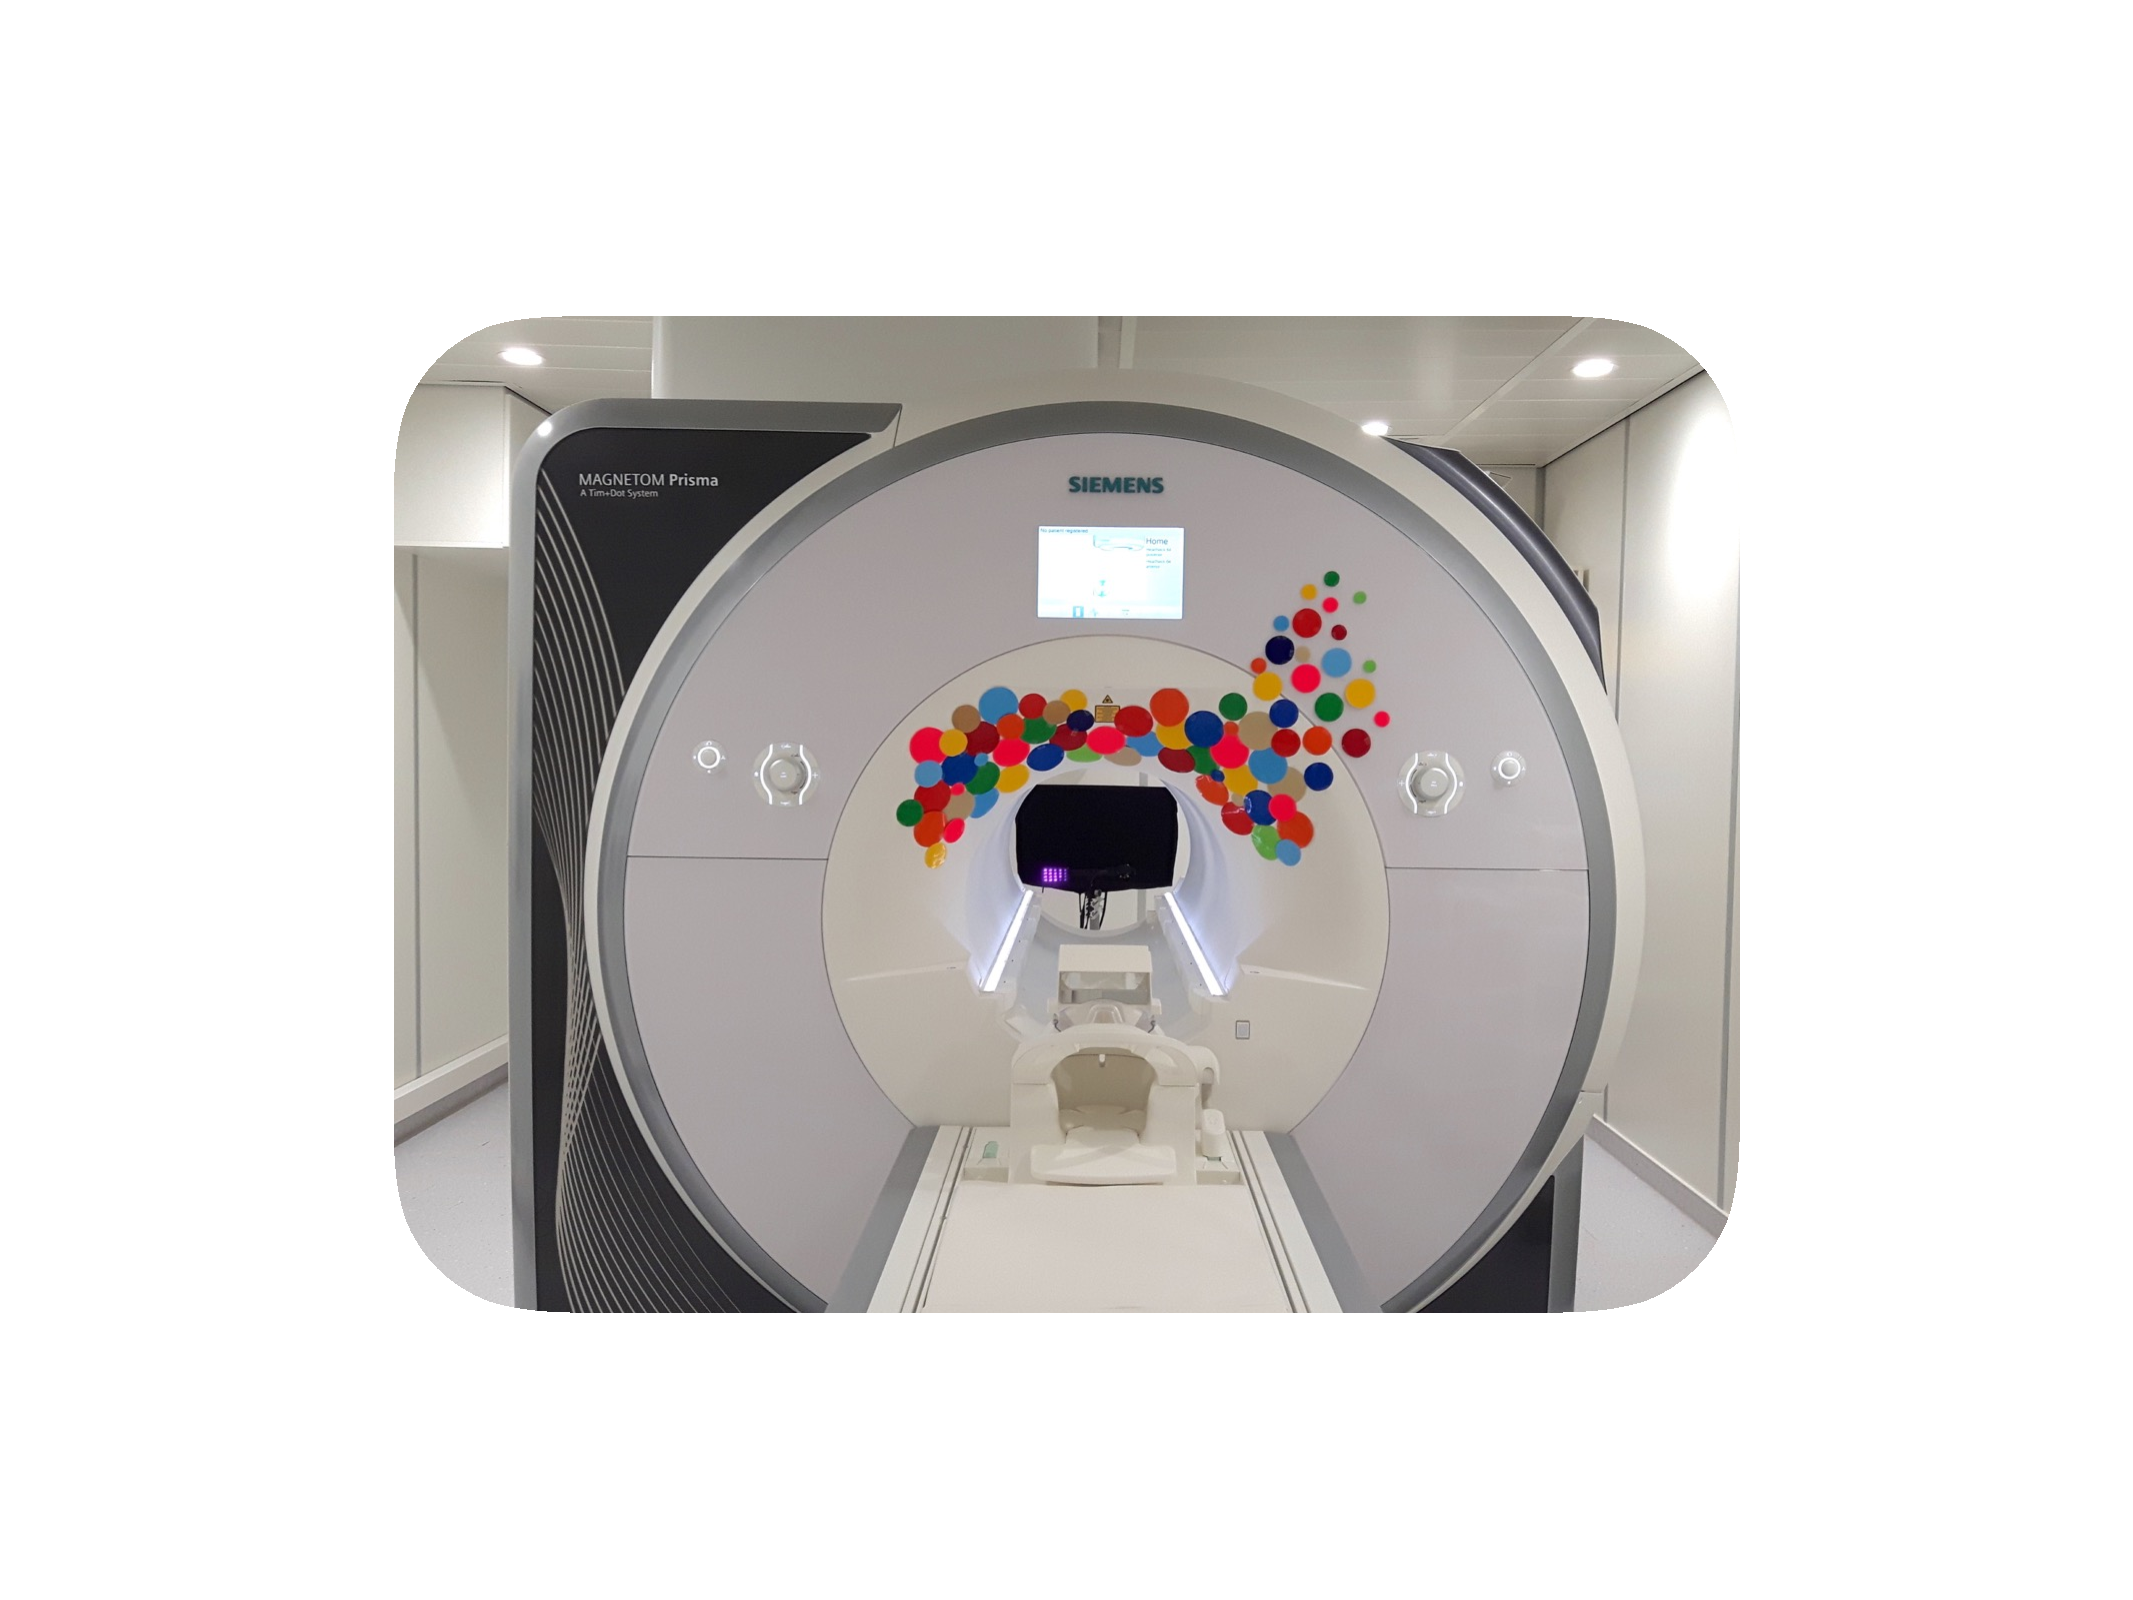
\includegraphics[width=1\linewidth]{images/Ch2/Ch2_MRI.pdf}
\caption{\textbf{The MRI machine at Campus Biotech, decorated with stickers to make the environment more child-friendly.} Approaches to familiarise children with the scanning environment have been shown to benefit data acquisition, resulting in better quality data that is less affected by motion-related artefacts.} \label{fig:MRI}
\end{figure}




Despite the increasing application of fMRI studies in infants, for example, the deployment and interpretation of such investigations in neonatal populations also remain a challenge. 
This is partly due to our still relatively limited understanding of the effects of brain development on the BOLD signal. 
It has been shown that the haemodynamic response changes during development, a phenomenon probably related to differences in neurovascular coupling at each stage \citep{Arichi2012}. 
Furthermore, the accuracy of task-based fMRI studies highly depends on the choice of HRF models: it has been shown that even small amounts of inaccuracy in HRF modeling may cause significant loss in validity and power \citep{Lindquist2007, Loh2008}. 
While \citeauthor{Arichi2012} (\citeyear{Arichi2012}) have shown differences in the response elicited in the somatosensory cortex of adults, termborn, and preterm children, age-appropriate HRF parameters (as well as its inter-region variability) are still to be firmly established.


Existing brain templates and atlases are typically based on adult brains and thus not optimised for spatial normalization and parcellation of infant data and small children.
Using them might thus reduce the accuracy of any quantitative analysis and generate mislocalisations in some cases. 
While several volumetric atlases have been proposed \citep{Habas2010, Kazemi2007, Shi2014}, no approach has been widely agreed upon since most obscure important spatial relationships among nearby locations in the cortex by blurring key structures, potentially leading to less accurate results \citep{Li2016}. 
Until spatial locations are well defined in the infant brain, analytical methods that do not rely on atlasing are more suitable for this population. For the young adolescents whose data were analysed in this thesis, we used a Montreal Neuroimaging Institute (MNI) template based on adult brains, as this has been consistently and successfully used in children above 7 years old  \citep{ASHBURNER1998, Burgund2002}. 

Finally, a recent review by \citet{Smid2016} has highlighted that, although most of the global preterm birth disease burden is on the shoulders of low and middle income countries (LMICs), only a very limited amount of research evidence for its prevention or treatment comes from studies in these settings. Instead, most of the research available on this population comes from high income countries and may thus offer an incomplete view of the global issue of preterm birth. Primary research involving LMICs thus also remains urgently needed. Nonetheless, research carried out in developed countries such as this one may still bring us closer to the development of interventions for which the need for expensive equipment will prove less essential, and LMIC populations will also benefit from them.  
